\documentclass{cs-mpi}
\graphicspath{{img/}}
\uleft{mpi* 2023}
\ucent{}
\uright{mini tutoriel \LaTeX{}}
\dleft{}
\dcent{\thepage}
\dright{}
%=========================
\begin{document}
\title{\LaTeX{} en MPI}
%=========================
\section{Un peu d'histoire}
%
\TeX{} est un système logiciel libre de composition de documents, indépendant du matériel utilisé pour la visualisation ou l'impression. Il fut créé à partir de 1977 par le mathématicien et informaticien \emph{Donald Knuth}, excédé par la piètre qualité de la typographie des logiciels d'édition de l'époque. Il est principalement conçu pour l'édition de documents techniques et est largement utilisé par les scientifiques, particulièrement en mathématiques, physique, bio-informatique, astronomie et informatique. Il est également extensible et permet notamment l'édition de documents plus complexes (affiches, plaquettes publicitaires, partitions musicales\dots). 
\TeX{} vient de τεχ, début du mot τέχνη, tékhnê (« art, science », en grec ancien), et se prononce /tɛx/2 ou /tɛk/, au choix.
\begin{center}

\includegraphics[height=16mm]{latex.png}
\end{center}
\LaTeX{}  est un langage et un système de composition de documents. Il s'agit d'une collection de macrocommandes destinées à faciliter l'utilisation du « processeur de texte » \TeX{}.
\LaTeX{} permet de rédiger des documents dont la mise en page est réalisée automatiquement en se conformant du mieux possible à des normes typographiques. Une fonctionnalité distinctive de LaTeX est son mode mathématique, qui permet de composer des formules complexes.
\LaTeX{} est particulièrement utilisé dans les domaines techniques et scientifiques pour la production de documents de taille moyenne (tels que des articles) ou importante (thèses ou livres, par exemple). Néanmoins, il peut être employé pour générer des documents de types très variés (lettres ou transparents, par exemple). Enfin, de nombreux sites Internet — dont le texte est typiquement mis en forme par d’autres moyens — emploient un sous-ensemble de LaTeX pour composer notamment leurs formules mathématiques. 
\\[2mm]
Source : \url{https://fr.wikipedia.org/wiki/TeX}
\\
Source : \url{https://fr.wikipedia.org/wiki/LaTeX}
%=========================
\section{Avant de commencer}
Deux options s'offrent à vous pour coder en \TeX{}. En pratique, vous coderez en \LaTeX{} et compilerez avec le moteur \codec{XeLaTeX} ou le moteur \codec{LuaLaTeX}.
\begin{itemize}
\item
Installer le système complet sur votre machine personnelle. Plus d'informations à ce sujet sont disponibles ici : \url{https://tug.org/texlive/}/
\item
Utiliser un système en ligne qui évite toute installation sur sa machine. Overleaf propose un tel service, gratuit pour un usage personnel : \url{https://fr.overleaf.com/}.
\end{itemize}
\begin{center}
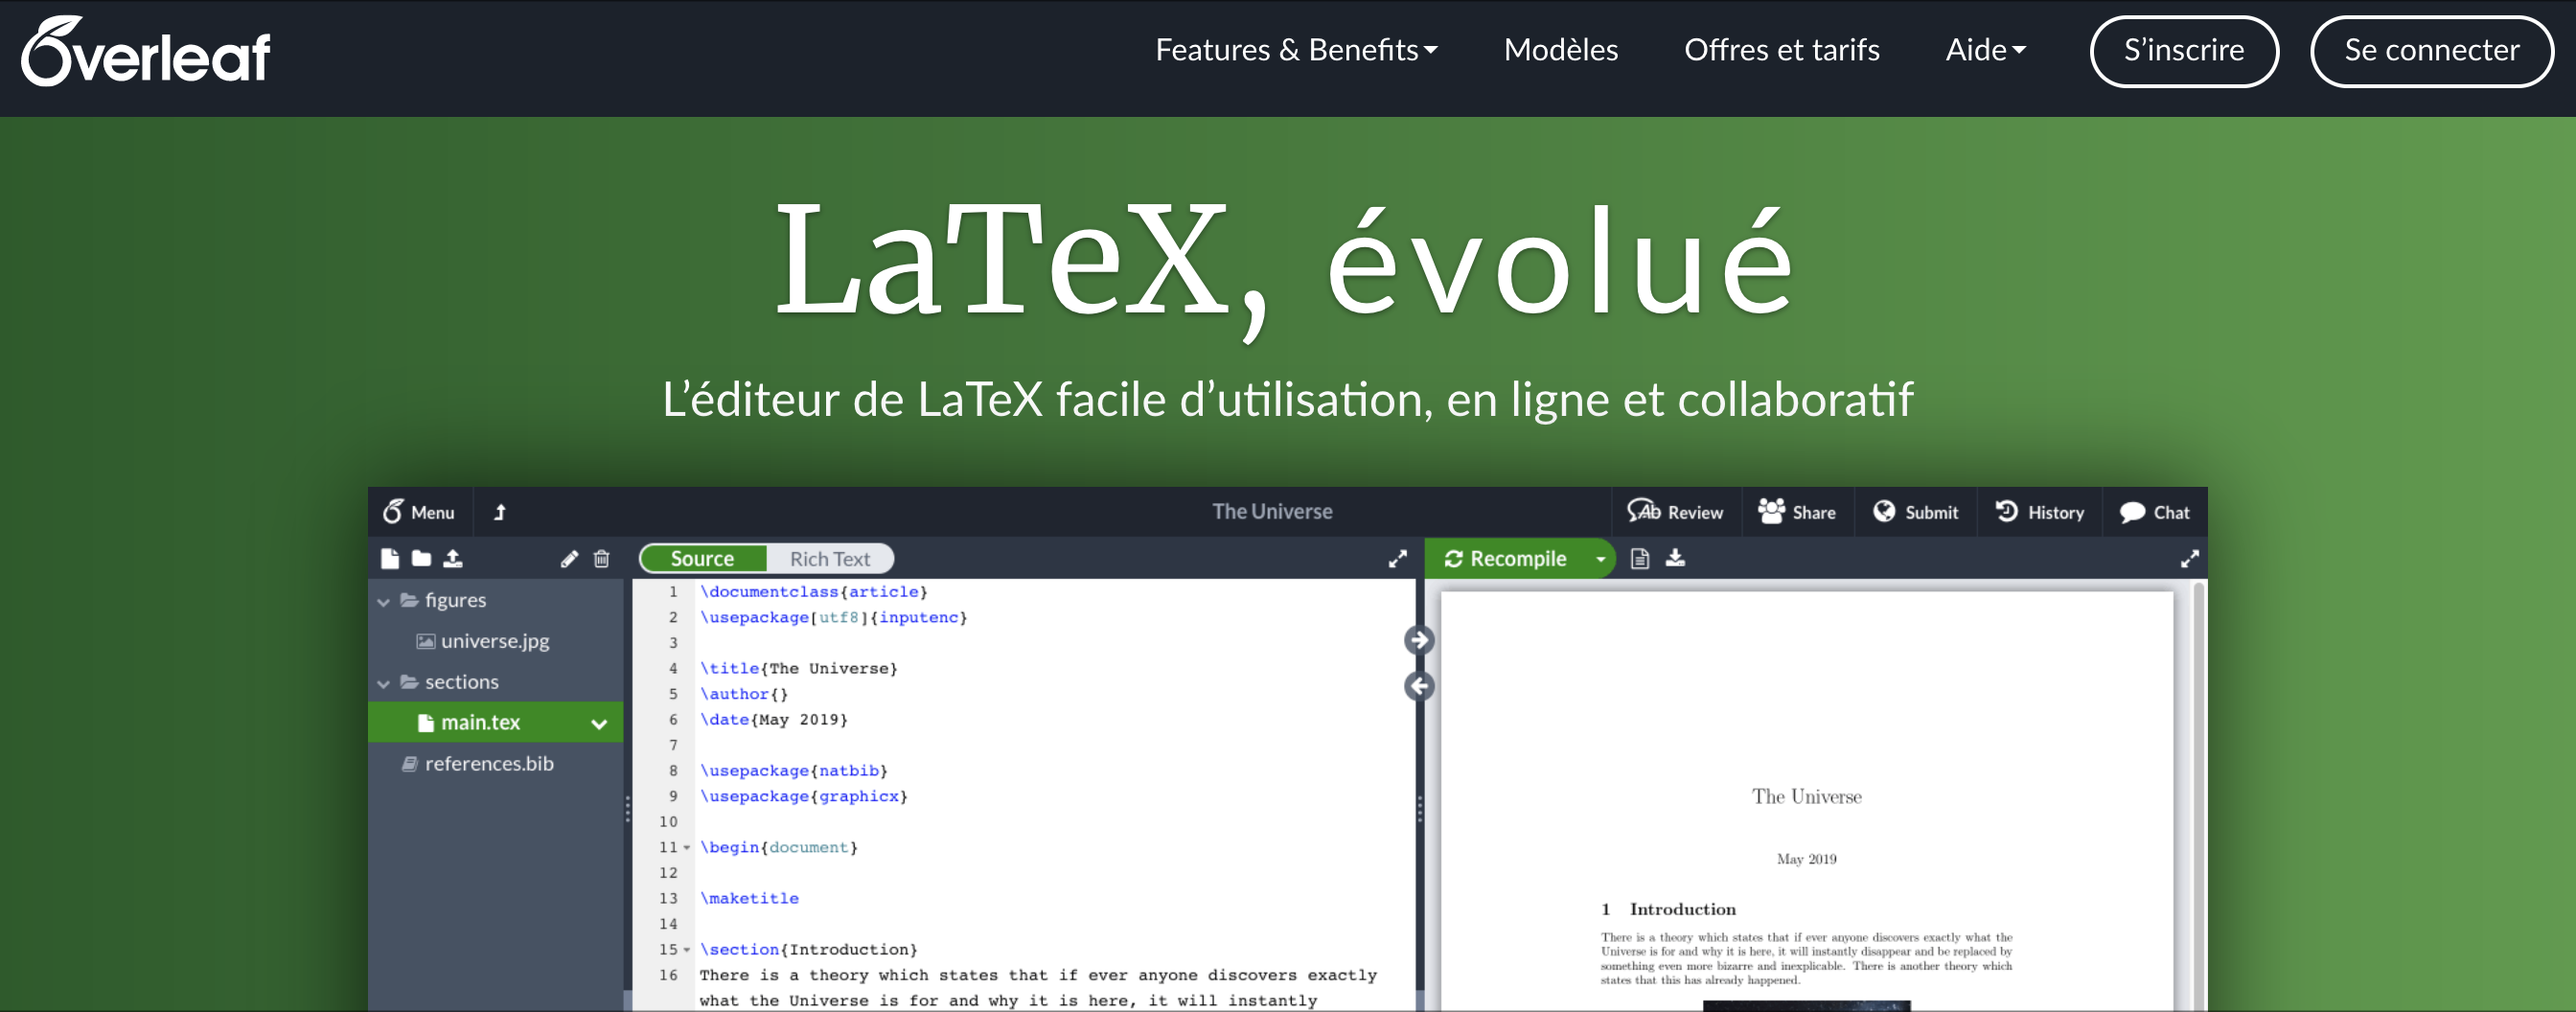
\includegraphics[width=\textwidth]{overleaf.png}
\end{center}
Pour vous aider dans la mise en page de documents de type rapport ou diaporamas, plusieurs fichiers sont à votre disposition. Il suffit de les déposer dans le même dossier que le fichier source de votre travail. Il est possible de les déposer dans un dossier spécifique (\code{localtexmf}) mais cette solution est pour les plus avertis. Selon que vous souhaitez écrire un rapport ou un diaporama, le squelette de votre fichier source aura toujours l'une des formes minimales suivantes.
\begin{multicols}{2}
\begin{tcblisting}{listing only}
\documentclass{cs-mpi}
\graphicspath{{img/}}
\uleft{mpi* 2023}
\ucent{}
\uright{en haut à droite}
\dleft{}
\dcent{\thepage}
\dright{}
%=========================
\begin{document}
%
% partie à compléter
%
%=========================
\end{document}
\end{tcblisting}
%
\begin{tcblisting}{listing only}
\documentclass{cs-mpi-diapo}
\graphicspath{{img/}}
%=========================
\begin{document}
%
% partie à compléter
%
%=========================
\end{document}
\end{tcblisting}
\end{multicols}
Le source est compilé en utilisant le moteur \codec{XeLaTeX} ou le moteur \codec{LuaLaTeX}. Bien s'assurer que cette option est activée au moment de la compilation qui fournit alors un document pdf en sortie.
%=========================
\section{Écrire en \LaTeX{}}
%-------------------------
\subsection{Du texte}
%
\begin{tcblisting}{listing side text}
\begin{defn}{}
Ceci est une définition.
\end{defn}
\begin{thm}{}
Ceci est un théorème.
\end{thm}
\begin{prop}{}
Ceci est une proposition.
\end{prop}
\begin{lem}{}
Ceci est un lemme.
\end{lem}
\begin{cor}{}
Ceci est un corollaire.
\end{cor}
\begin{exemple}{}
Ceci est un exemple.
\end{exemple}
%
\begin{rem}
Ceci est une remarque.
\end{rem}
\begin{demo}
Ceci est une démonstration
\end{demo}
\end{tcblisting}
%
\begin{tcblisting}{breakable}
\begin{defn}{problème de l'arrêt en OCaml}
Le \emph{problème de l'arrêt} consiste à écrire une fonction OCaml :
\\
\centerline{\codec{halt: string -> string -> bool}}
prenant en entrées :
\begin{itemize}
\item une chaîne \codec{f} contenant le code source d'un programme OCaml,
\item une chaîne \codec{e} représentant des entrées pour le programme donné par \codec{f},
\end{itemize}
et qui, pour toutes chaînes \codec{f} et \codec{e}, termine en un temps fini en renvoyant \codec{true} si l'exécution du programme \codec{f} sur les entrées \codec{e} termine en temps fini, et \codec{false} sinon.
\end{defn}
\end{tcblisting}
%
\begin{tcblisting}{breakable}
Ce problème n'a pas de solution algorithmique : il est \emph{indécidable}.
%
\begin{thm}{}
Il n'existe pas de fonction OCaml résolvant le problème de l'arrêt.
\end{thm}
\end{tcblisting}
%
\begin{tcblisting}{breakable}
\begin{demo}
La démonstration procède par l'absurde.
Supposons l'existence d'une fonction \codec{halt} répondant à la spécification du problème de l'arrêt et considérons alors la fonction \codec{weird} suivante.
\begin{ocaml}
let weird f e =
  if halt f e then
    while true do print_string "ok" done;
\end{ocaml}
Cette fonction reçoit les arguments \codec{f} et \codec{e} puis teste, par l'appel à la fonction \codec{halt}, l'arrêt de l'exécution du programme \codec{f} sur les entrées \codec{e}.
\begin{itemize}
\item
Si cet appel renvoie \codec{true}, c'est que l'exécution de \codec{f} sur \codec{e} s'arrête effectivement. La fonction \codec{weird} entre dans une boucle infinie et ne s'arrête jamais. 
\item
Si cet appel renvoie \codec{false}, c'est que l'exécution de \codec{f} sur \codec{e} ne s'arrête pas. La fonction \codec{weird} ne fait alors rien et s'arrête immédiatement.
\end{itemize}
Ainsi \codec{weird f e} s'arrête si et seulement \codec{halt f e} ne s'arrête jamais.

Considérons à présent la fonction \codec{paradox}.
\begin{ocaml}
let paradox g = weird g g
\end{ocaml}
Alors \codec{paradox f} s'arrête uniquement si et seulement si l'exécution de \codec{f} sur \codec{f} ne s'arrête jamais.

Appliquons cette fonction à elle-même. En vertu de ce qui vient d'être établi, \codec{paradox paradox} s'arrête si et seulement si \codec{paradox paradox} ne s'arrête jamais ! Résultat qui établit clairement une équivalence entre une proposition et sa négation et constitue, de fait, une contradiction.

En conséquence, l'existence de la fonction \codec{paradox} est contradictoire et, en remontant la chaîne des fonctions ayant mené à sa définition, celle de la fonction \codec{halt} l'est aussi. Il n'existe donc pas de fonction \codec{halt}. Le problème de l'arrêt est \emph{indécidable}.
\end{demo}
\end{tcblisting}
%-------------------------
\subsection{Des mathématiques}
\begin{tcblisting}{}
Une suite $(u_{n})_{n\in\N}$ est définie par ses deux premiers termes $u_{0} = 0$ et $u_{1} = 1$ et, pour tout entier naturel $n$, par la relation de récurrence suivante.
\[ u_{n+2} = u_{n+1} + u_{n} \]
Il s'agit de la célèbre suite de Fibonacci\footnote{Qui s'appelait également Leonard de Pise.} dont l'expression générale peut s'écrire :
\[ \forall n \in \N 
\quad
u_n = \frac{1}{\sqrt{5}} \left( \varphi^{n} - \hat{\varphi}^{n} \right)
\]
avec $\varphi^{n} = (1 + \sqrt{5}) / 2$ et $\hat{\varphi}^{n} = (1 - \sqrt{5}) / 2$.
\end{tcblisting}
%-------------------------
\subsection{Du code}
%
\begin{tcblisting}{breakable, listing side text}
Le fichier de configuration propose deux instructions pour saisir du code en ligne : \code{let x = 2} (en N\&B) et \codec{let x = 2} (en couleur).
Un bloc de code peut être saisi entre comme suit.
%
\begin{ocaml}
(* code OCaml *)
let smart_not f = match f with
  | True  -> False
  | False -> True
  | _     -> Not f
\end{ocaml}
%
\begin{C}
// Code C
struct bloc {
  void *adresse;
  uint32_t taille;
  bool libre;
  struct bloc *suivant;
};
\end{C}
\end{tcblisting}
%-------------------------
\subsection{Du graphisme}
Il est possible de créer des graphiques en les programmation. \emph{PGF/TikZ} est une combinaison de deux langages informatiques permettant la création de graphiques vectoriels. \emph{PGF} est un langage de bas niveau, tandis que \emph{TikZ} est un ensemble de macros qui fournit une syntaxe plus simple comparée à celle de PGF. Ce dernier est très utilisé dans le monde \TeX{} mais sa maîtrise requiert quelques heures de travail. Le résultat est cependant de très grande qualité. Voir les sites \url{https://tikz.net/}, \url{https://tikz.dev/} et le document \url{http://math.et.info.free.fr/TikZ/bdd/TikZ-Impatient.pdf}.
%
\begin{tcblisting}{breakable}
\tikzstyle{every path} = [> = stealth', shorten > = 1pt, line width=1pt]
\tikzstyle{state} = [circle, fill=white, draw=black, text=black, minimum width=2mm, minimum size=6mm, inner sep=0pt, node distance=16mm, line width=1pt]
\tikzstyle{init} = [initial, initial text=]
\tikzstyle{term} = [accepting]
\begin{center}
\begin{tikzpicture}
\node[state, init, term] (0) {$0$};
\node[state, right of=0] (1) {$1$};
\node[state, right of=1] (2) {};
\node[state, right of=2, draw=white] (dots) {$\dots$};
\node[state, right of=dots] (n1) {};
\node[state, right of=n1] (n) {$n$};
\path[->]
(0) edge[bend left] node[above]{$a$} (1)
(1) edge[bend left] node[above]{$a$} (2)
    edge[bend left] node[below]{$b$} (0)
(2) edge[bend left] node[above]{$a$} (dots)
    edge[bend left] node[below]{$b$} (1)
(dots) edge[bend left] node[above]{$a$} (n1)
    edge[bend left] node[below]{$b$} (2)
(n1) edge[bend left] node[above]{$a$} (n)
    edge[bend left] node[below]{$b$} (dots)
(n) edge[bend left] node[below]{$b$} (n1)
;
\end{tikzpicture}
\end{center}
\end{tcblisting}
%
\begin{tcblisting}{listing side text}
Une autre solution est de créer des graphiques à l'aide de logiciels dédiés puis d'exporter le résultat dans un fichier image. Ce dernier peut être inclus dans un document \LaTeX{} par la commande \codec{includegraphics}.
\begin{center}
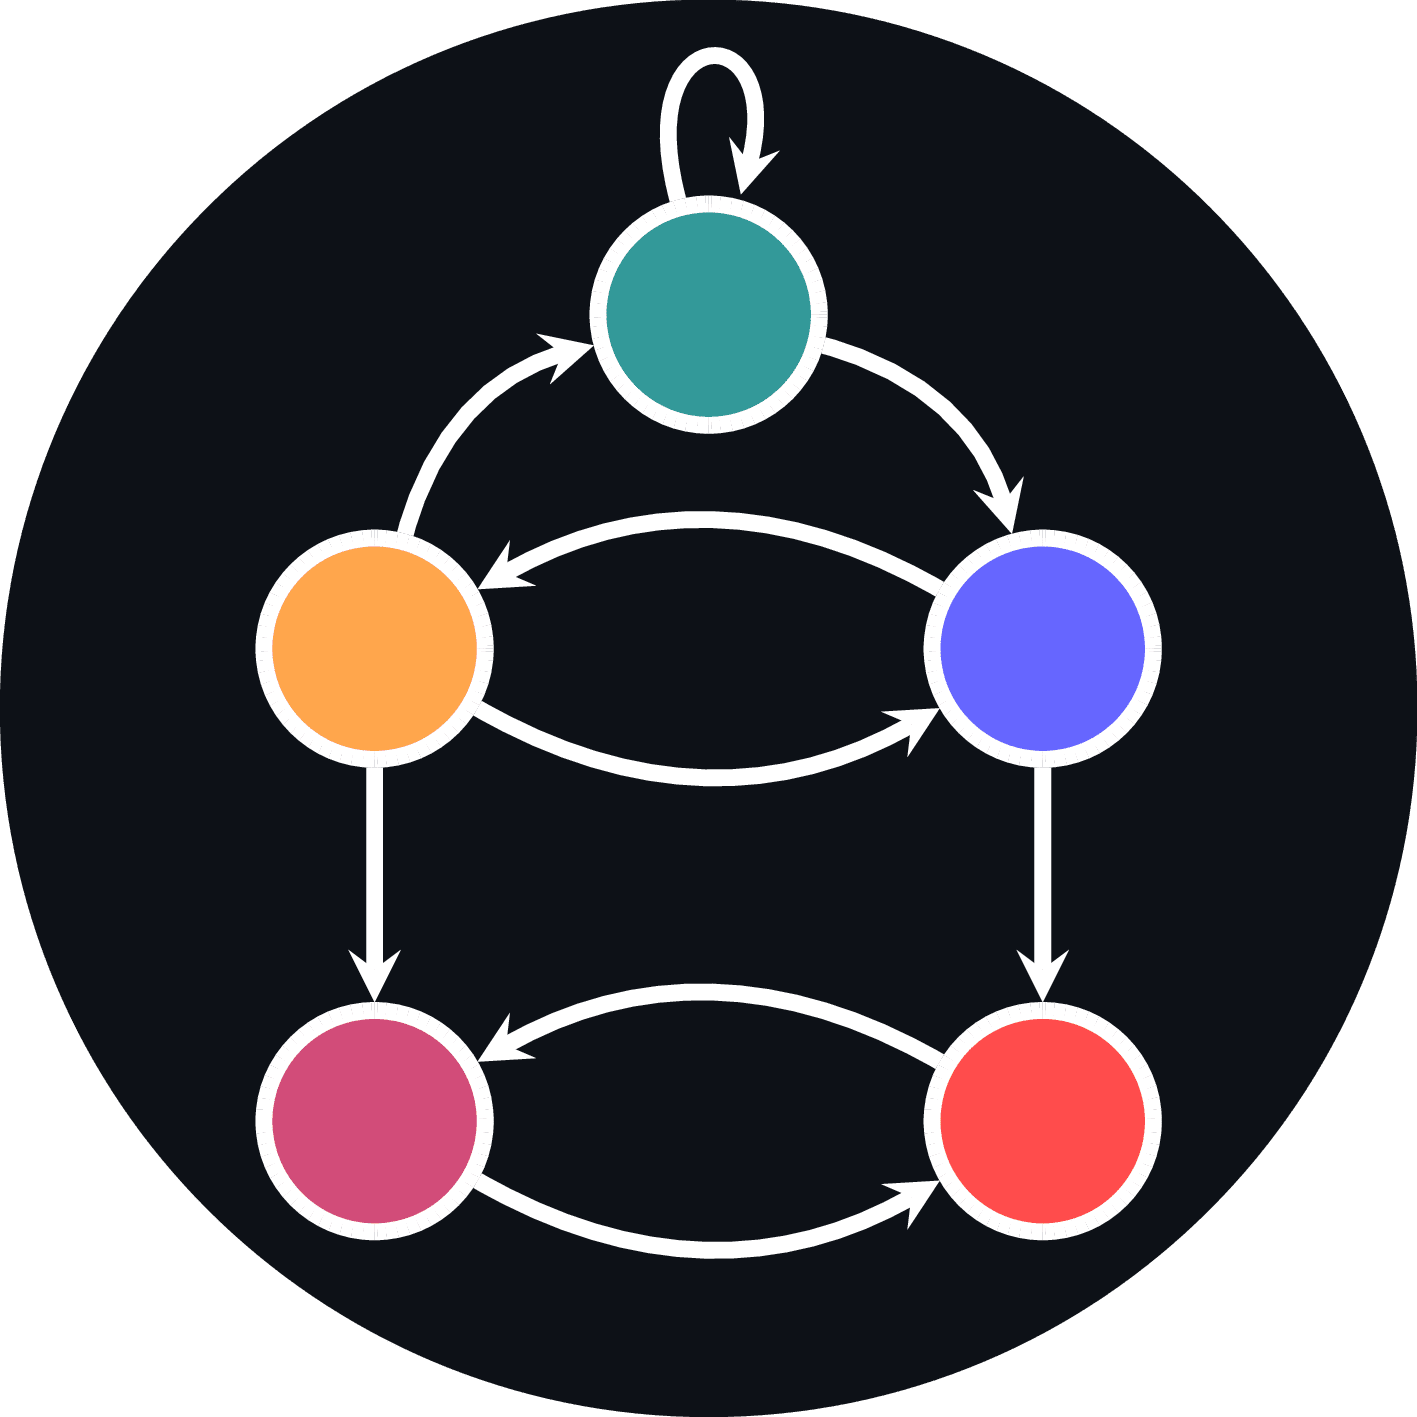
\includegraphics[height=32mm]{img/aviary.png}
\end{center}
\end{tcblisting}
%-------------------------
\subsection{Des questions}
\begin{tcblisting}{listing side text}
\question
Qu'est l'informatique ?
%
\question
Un ordinateur peut-il résoudre tous les problèmes de décision ?
%
\question
Présenter brièvement un algorithme qui effectue les calculs suivants.
\squestion
Recherche dichotomique dans un tableau
\squestion
Exponentiation rapide
\squestion
Parcours en profondeur d'abord d'un graphe
\squestion
Détermination d'un arbre couvrant minimal
\end{tcblisting}
%=========================
\end{document}